\section{Конструкторский раздел }

В данном разделе описаны основные объекты, используемые в системе.

\subsection{Основные структуры}

Для реализации программной системы был выбран язык программирования Python.  В качестве СУБД была использована MySQL. 

Используемые в системе классы: 
\begin{enumerate}
\itemатрибуты (Attribute);
\itemтаблица (Table);
\itemдомен (Domen);
\itemмножество всех доменов (DomenSearch);
\itemмножество оптимальных доменов (OptimalDomen).
\end{enumerate}

\begin{figure}[H]
\center{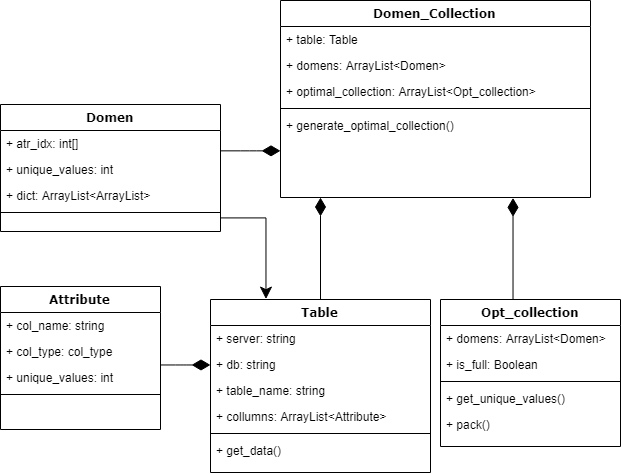
\includegraphics[width = 0.8\linewidth]{class_d}}
\caption{Диаграмма классов}
\end{figure}

Класс атрибута описывает столбец обрабатываемой таблицы. Класс содержит имя столбца, тип данных, который он содержит, а также количество уникальных значений. 
\\

\begin{figure}[H]
\lstinputlisting{attribute.py}
\caption{Класс атрибута}
\end{figure} 
 

Класс таблицы описывает обрабатываемую таблицу. Класс содержит имя столбца, её размер, а также лист атрибутов-столбцов. Помимо этого класс содержит методы получения данных.
\\

\begin{figure}[H]
\lstinputlisting{table.py}
\caption{Класс таблицы}
\end{figure} 

Класс домена описывает наименьший основной фрактальный объект, домен. Класс содержит лист индексов входящих в него атрибутов-столбцов, а также количество уникальных значений в данном домене. Класс включает в себя метод получения количества уникальных значений.
\\

\begin{figure}[H]
\lstinputlisting{domen.py}
\caption{Класс домена}
\end{figure} 
 
Класс множества всех доменов описывает алгоритмы работы с множеством доменов. Класс содержит лист индексов входящих в него атрибутов-столбцов, а также количество уникальных значений в данном домене. Класс включает в себя метод получения количества уникальных значений.

\begin{figure}[H]
\lstinputlisting{domen_collection.py}
\caption{Класс домена}
\end{figure} 
  

\pagebreak